\chapter{Case studies}
\label{chp:case_studies}
% ---------------------------------------------------------------------------------------------------

% ===================================================================================================
\section{A mechanistic emulator: learning the \emph{weir equation}}
% ===================================================================================================

% ---------------------------------------------------------------------------------------------------
\subsection{Material and methods}
% ---------------------------------------------------------------------------------------------------

% ---------------------------------------------------------------------------------------------------
\subsection{Results and discussion}
% ---------------------------------------------------------------------------------------------------


% ===================================================================================================
\newpage
\section{An hydrological emulator: estimating the time-to-peak}
% ===================================================================================================



With this case study it was decided to address a complex hydrological problem by means of emulation.
The problem we want to solve is estimating the time needed for a channel conveying water from a catchment to reach a certain threshold discharge ($Q_!$) at its outlet as a function of rain intensity and initial soil saturation.

For the experiment a synthetic catchment topography was used, which at first glance can make the case study look very abstract.
In reality the emulator is just exploiting the catchment specific behavior, which is of course different from one catchment to another, but the methodology applied here could be applied to whatever catchment.
The emulator developed here, with the appropriate adjustments, could maybe be exploited as an \emph{early flood warning tool}.

% ---------------------------------------------------------------------------------------------------
\subsection{Material and methods}
% ---------------------------------------------------------------------------------------------------

\subsubsection{Generating the synthetic topography}

As for the previous example, the simulations were run with the open source software \textit{FullSWOF\_2D-v.1.07.00} \autocite{delestre_fullswof:_2014} \noteseb{put the citation every time that it is mentioned?}, while the input files necessary for the simulations were prepared with \textit{GNU Octave 4.2.1} \autocite{octave_community_gnu_2018} \noteseb{how to cite this?} with the aid of the package \textit{fswof2d}.

The topography used represents a catchment of size $\SI{2}{\kilo\meter} \times \SI{2}{\kilo\meter}$ and it is visible in Fig~\ref{fig:topography}.
It is composed of a sloping plane with three Gaussian bumps on the top.
The Gaussian bumps have different heights and widths and generate a \emph{Y-shaped channel} which extends from the upper and left boundary down to the lower boundary.
A paraboloid was added to the plane to promote the accumulation of water in the channel.
This has a single outlet located close to the center of the domain's bottom boundary.

The synthetic topography produced, in contrast to a real one, has the advantage of having a much smoother surface, which allows using a coarser grid resolution without losing topographical features.
The coarser the grid the fewer the nodes where FV equations have to be solved, which reduces the simulation runtime \noteseb{how does it decrease? linearly? quadratically?}. 
Another advantage of having a smooth topography, not presenting discontinuities, is that the solutions converge easily, and no grid refinement is necessary.
The grid used is composed of $\num{100} \times \num{100}$ cells, giving a resolution of $\SI{20}{\meter} \times \SI{20}{\meter}.$


\begin{figure}[htpb]
  \centering
  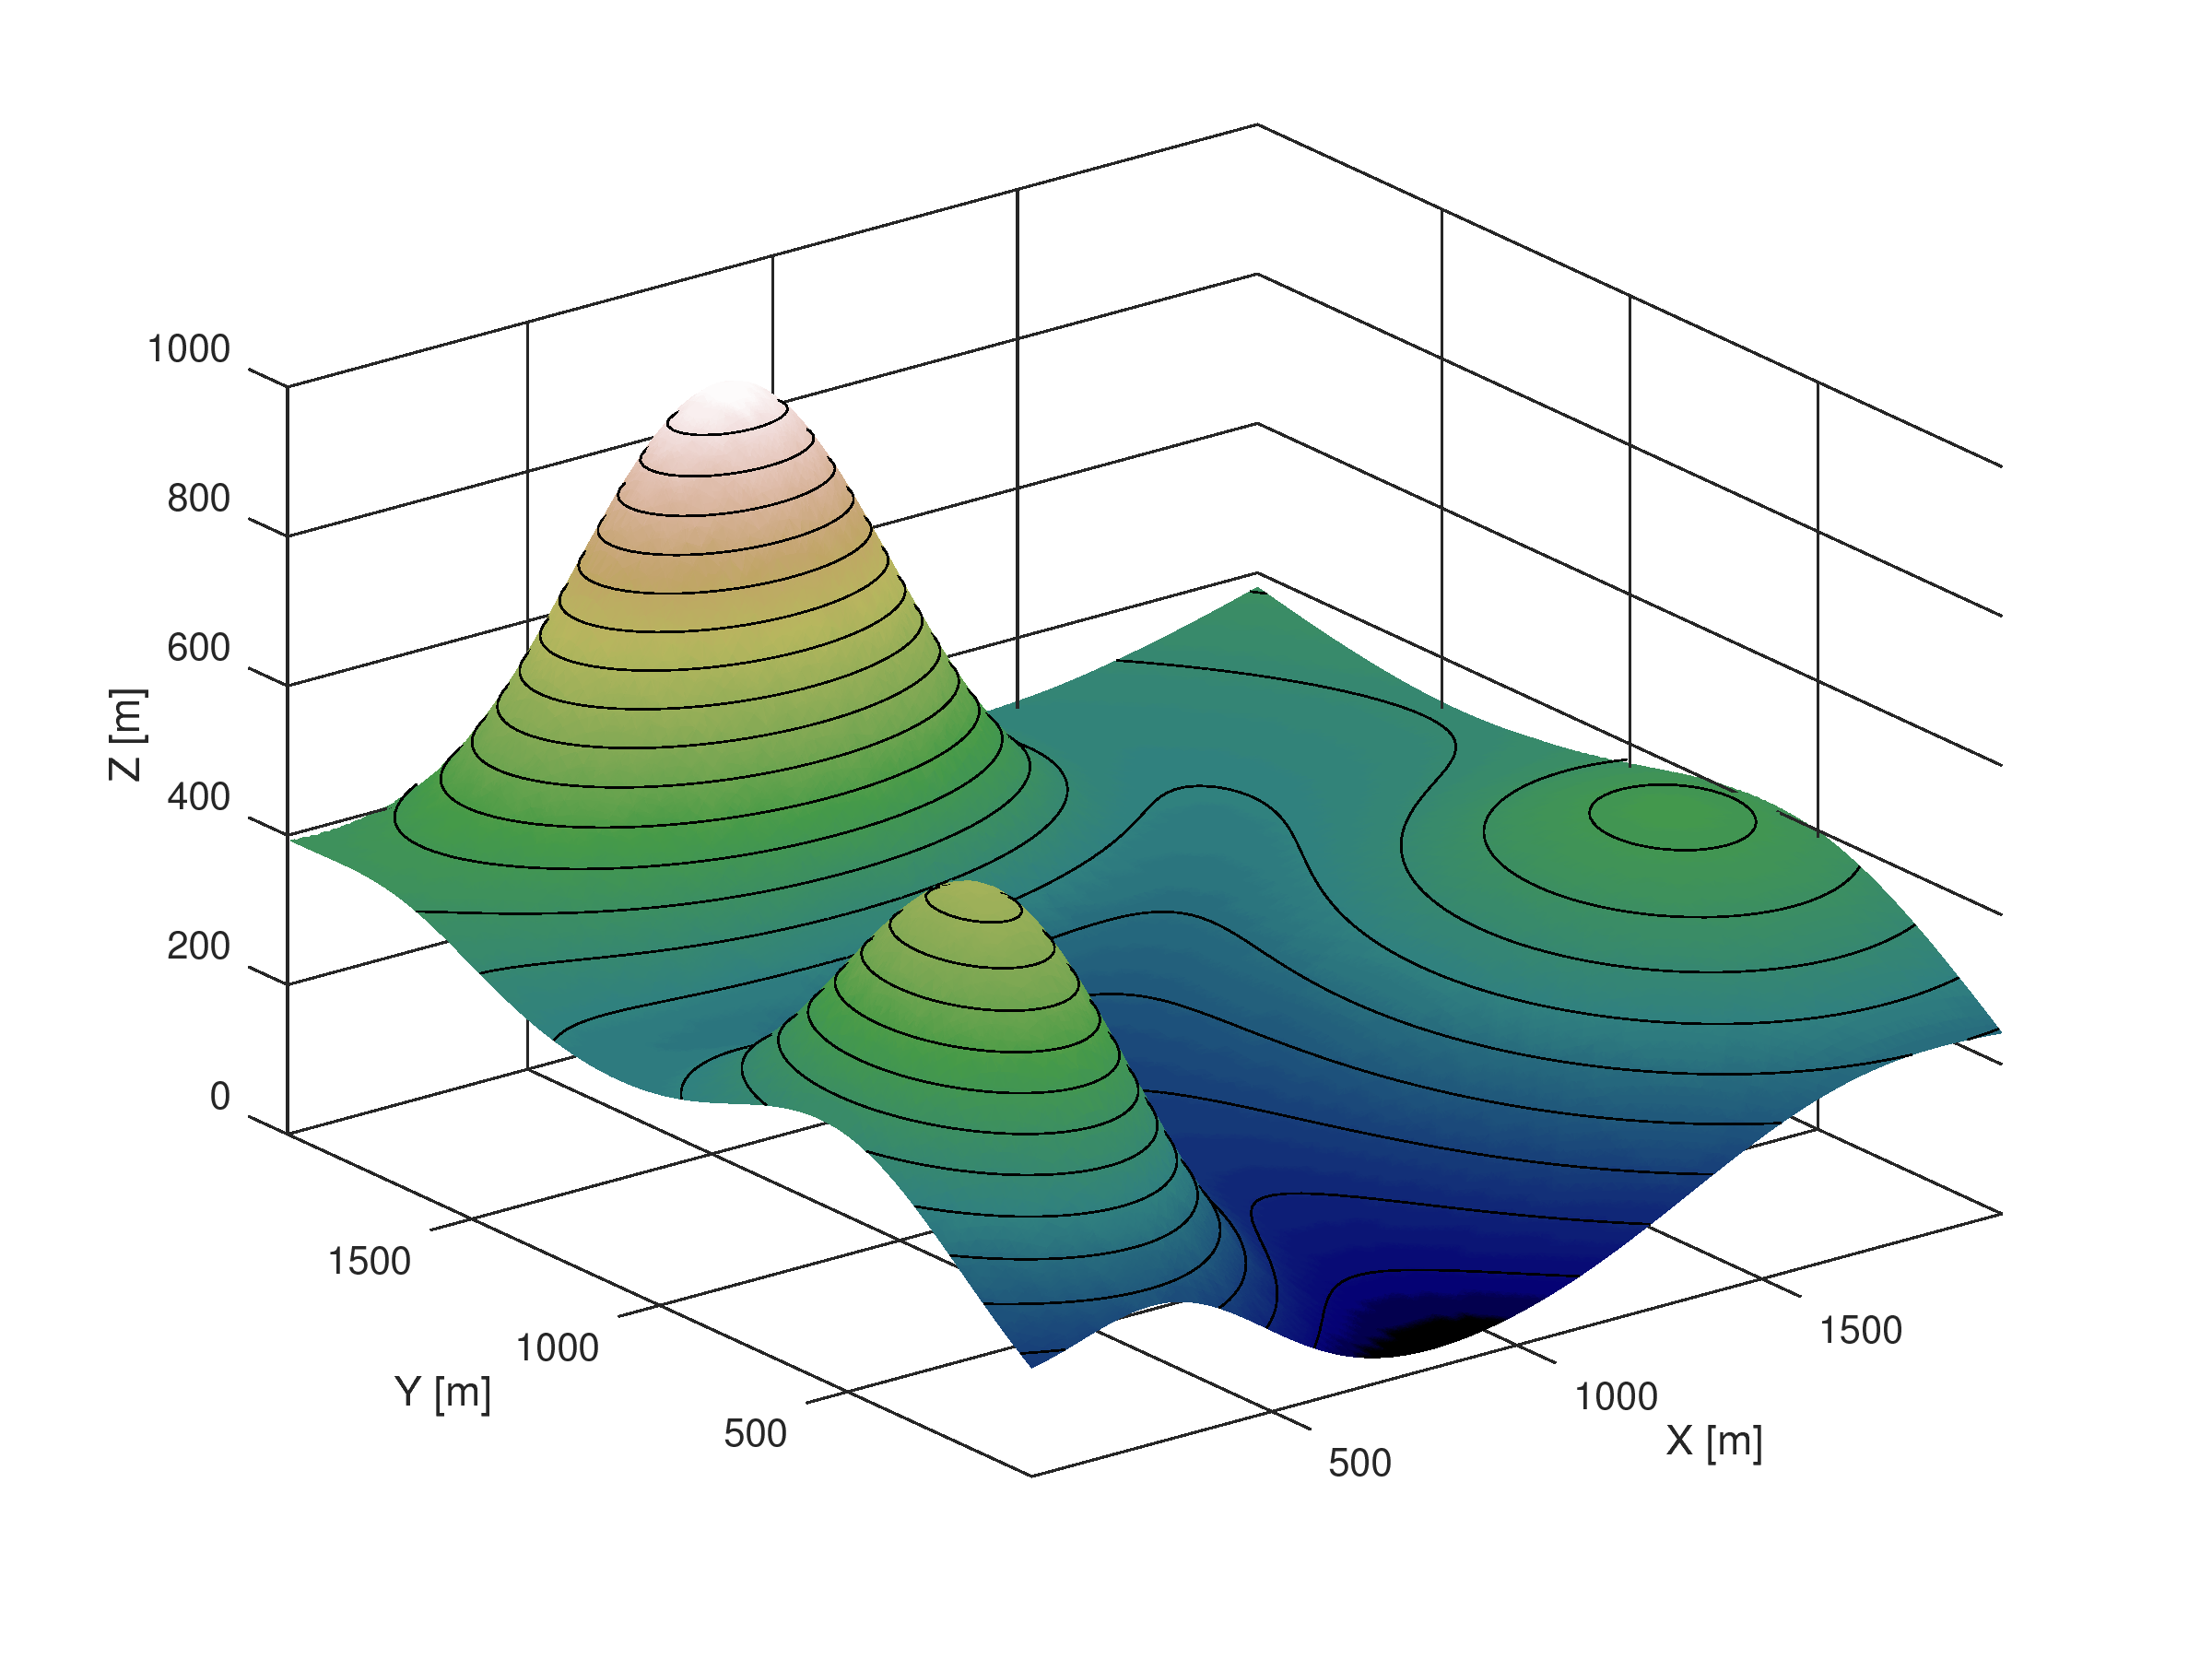
\includegraphics[width=0.7\textwidth]{Figures/topography.png}
  \caption{Synthetic topography composed of three Gaussian bumps on a sloping plane.}
  \label{fig:topography}
\end{figure}



\subsubsection{Setting-up the simulations}

The dataset required for building the emulator was generated by running \num{50} simulations with different combinations of the variables \emph{rain intensity} ($I$) and \emph{initial soil saturation} ($\theta_i$).
The initial soil saturation, being a spatially distributed variable, was kept uniform over the whole domain.
The rain intensity was kept constant and was uniformly applied over the domain, also since \textit{FullSWOF\_2D}, at this stage of development, only allows for uniformly distributed rain events.

\num{5} different initial saturations in the $[\numrange{0}{1}]$ interval and \num{10} rain intensities in the \SIrange{10}{35}{\milli\metre\per\hour} interval were taken and all their possible combinations were used as inputs for the simulations.
The rain duration was set to \SI{6}{\hour}, while a simulation duration of \SI{9}{\hour} was chosen in order to be able to observe the hydrograph recession. A time resolution of \SI{60}{\second} was used, meaning that intermediate simulation results were written to the \emph{outputs} file every \SI{60}{\second}.

Some parameters, namely those specific for the catchment in questions, were kept constant over all of the simulations.
These are summarized in Tab.~\ref{tab:simulations_parameters}.
The parameters marked with * are those \emph{spatially distributed}, meaning that a different value could be set for every cell.
For simplicity, a spatially uniform catchment was used, therefore the values from the table are valid for the whole domain.
Three \textit{wall boundary conditions} were set, for the upper and the two lateral boundaries.
For the bottom boundary a \textit{Neumann boundary condition} was selected, allowing water to freely outflow through that boundary and making sure that all of the water is lost from here.




\begin{table}[htpb]
  \centering
  \caption{Parameters and setting fixed for all simulations.}
  \label{tab:simulations_parameters}
  \begin{threeparttable}
    \begin{tabular}{lrl}
      \toprule
      \textbf{Parameter} & \textbf{Value} & \textbf{Units} \\
      \midrule
      Domain x-length                          &    $2'000$           & \si{\meter}   \\
      Domain y-length                          &    $2'000$           & \si{\meter}   \\
      Number of cells x                        &    $100$             & --   \\
      Number of cells y                        &    $100$             & --   \\
      Friction coefficient\tnote{*}            &    $0.03$            & \si{s.m^{-1/3}}\\
      Crust thickness\tnote{*}                 &    $1$               & \si{\meter}\\
      Crust hydraulic conductivity\tnote{*}    &    $2\cdot 10^{-6}$  & \si{\meter\per\second}\\
      Soil hydraulic conductivity\tnote{*}     &    $2\cdot 10^{-6}$  & \si{\meter\per\second}\\
      Soil suction head\tnote{*}               &    $0.09$      & \si{\meter}\\
      Soil maximum infiltration rate\tnote{*}  &    $19.8$      & \si{\milli\meter\per\hour}\\
      \bottomrule
    \end{tabular}
    \begin{tablenotes}
      \item[*] Parameters spatially distributed.
    \end{tablenotes}
  \end{threeparttable}
\end{table}


\subsubsection{Extracting the datasets}

The datasets used to build the emulator had to be extracted from the simulation outputs

This data constitute the \emph{training} dataset for the emulator.
A \emph{test} dataset and a \emph{validation} dataset were also generated and can be found in the Appendix~\ref{Appendix}. \noteseb{verify if they are really added}


% ---------------------------------------------------------------------------------------------------
\subsection{Results and discussion}
% ---------------------------------------------------------------------------------------------------

\begin{itemize}
\itemsep0em
  \item emulator should never underestimate danger (what type of error is this? we want to avoid it absolutely)
  \item try to perform GP interpolation. If it does not work, explain why polynomial interpolation (no time)
  \item use emulator with uncertainty in the $I$ and $\theta_i$. Perform uncertainty quantification
\end{itemize}


\subsubsection{Classification emulator}

Results for the classification emulator
\begin{itemize}
  \item show classification with 3 different $Q_!$
  \item perform testing 
\end{itemize}

\begin{figure}[htpb]
  \centering
  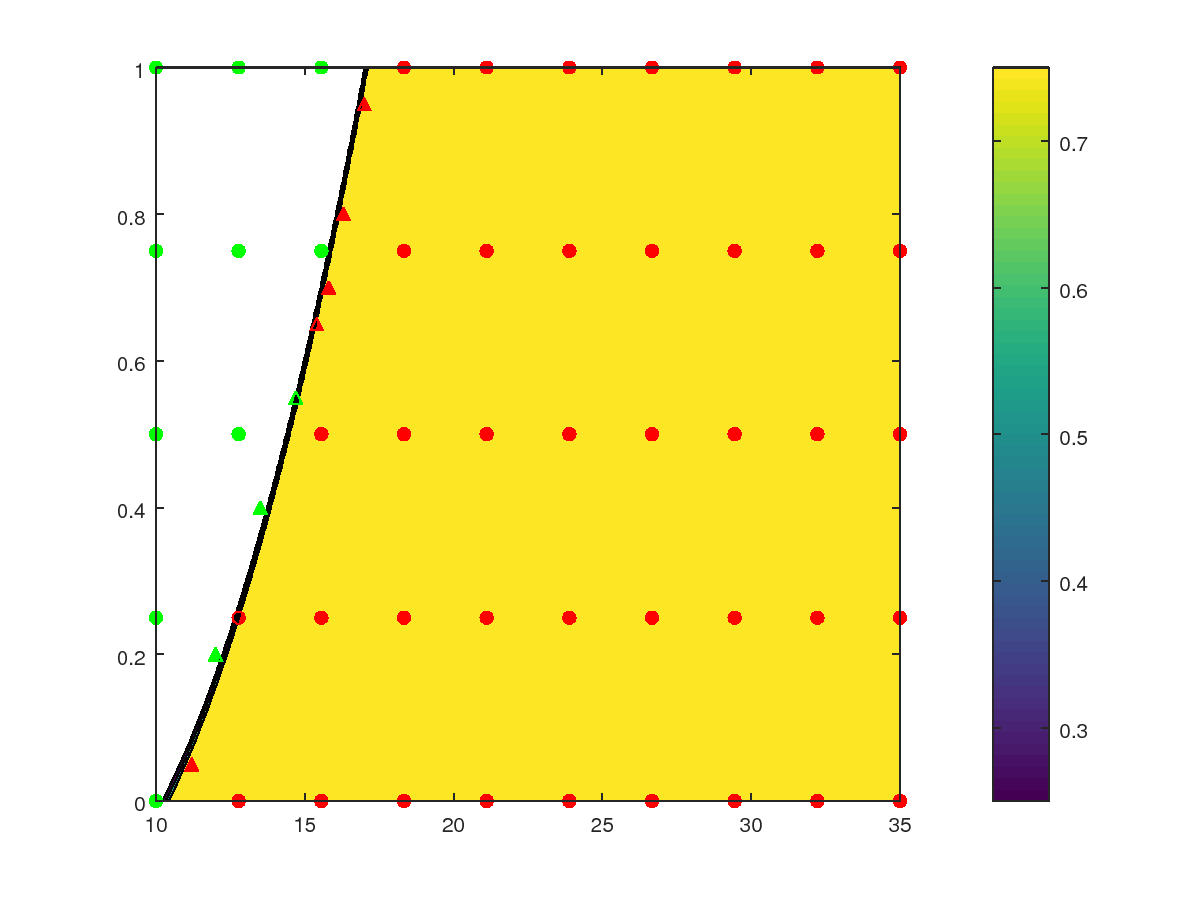
\includegraphics[width=0.75\textwidth]{Figures/classification.png}
  \caption{Binary classification emulator: events reaching $Q_!$ (red) and events not reaching $Q_!$ (green) for $Q_! = XX.X$.}
  \label{fig:classification_Q1}
\end{figure}


\subsubsection{Regression emulator}

\begin{figure}[htpb]
  \centering
  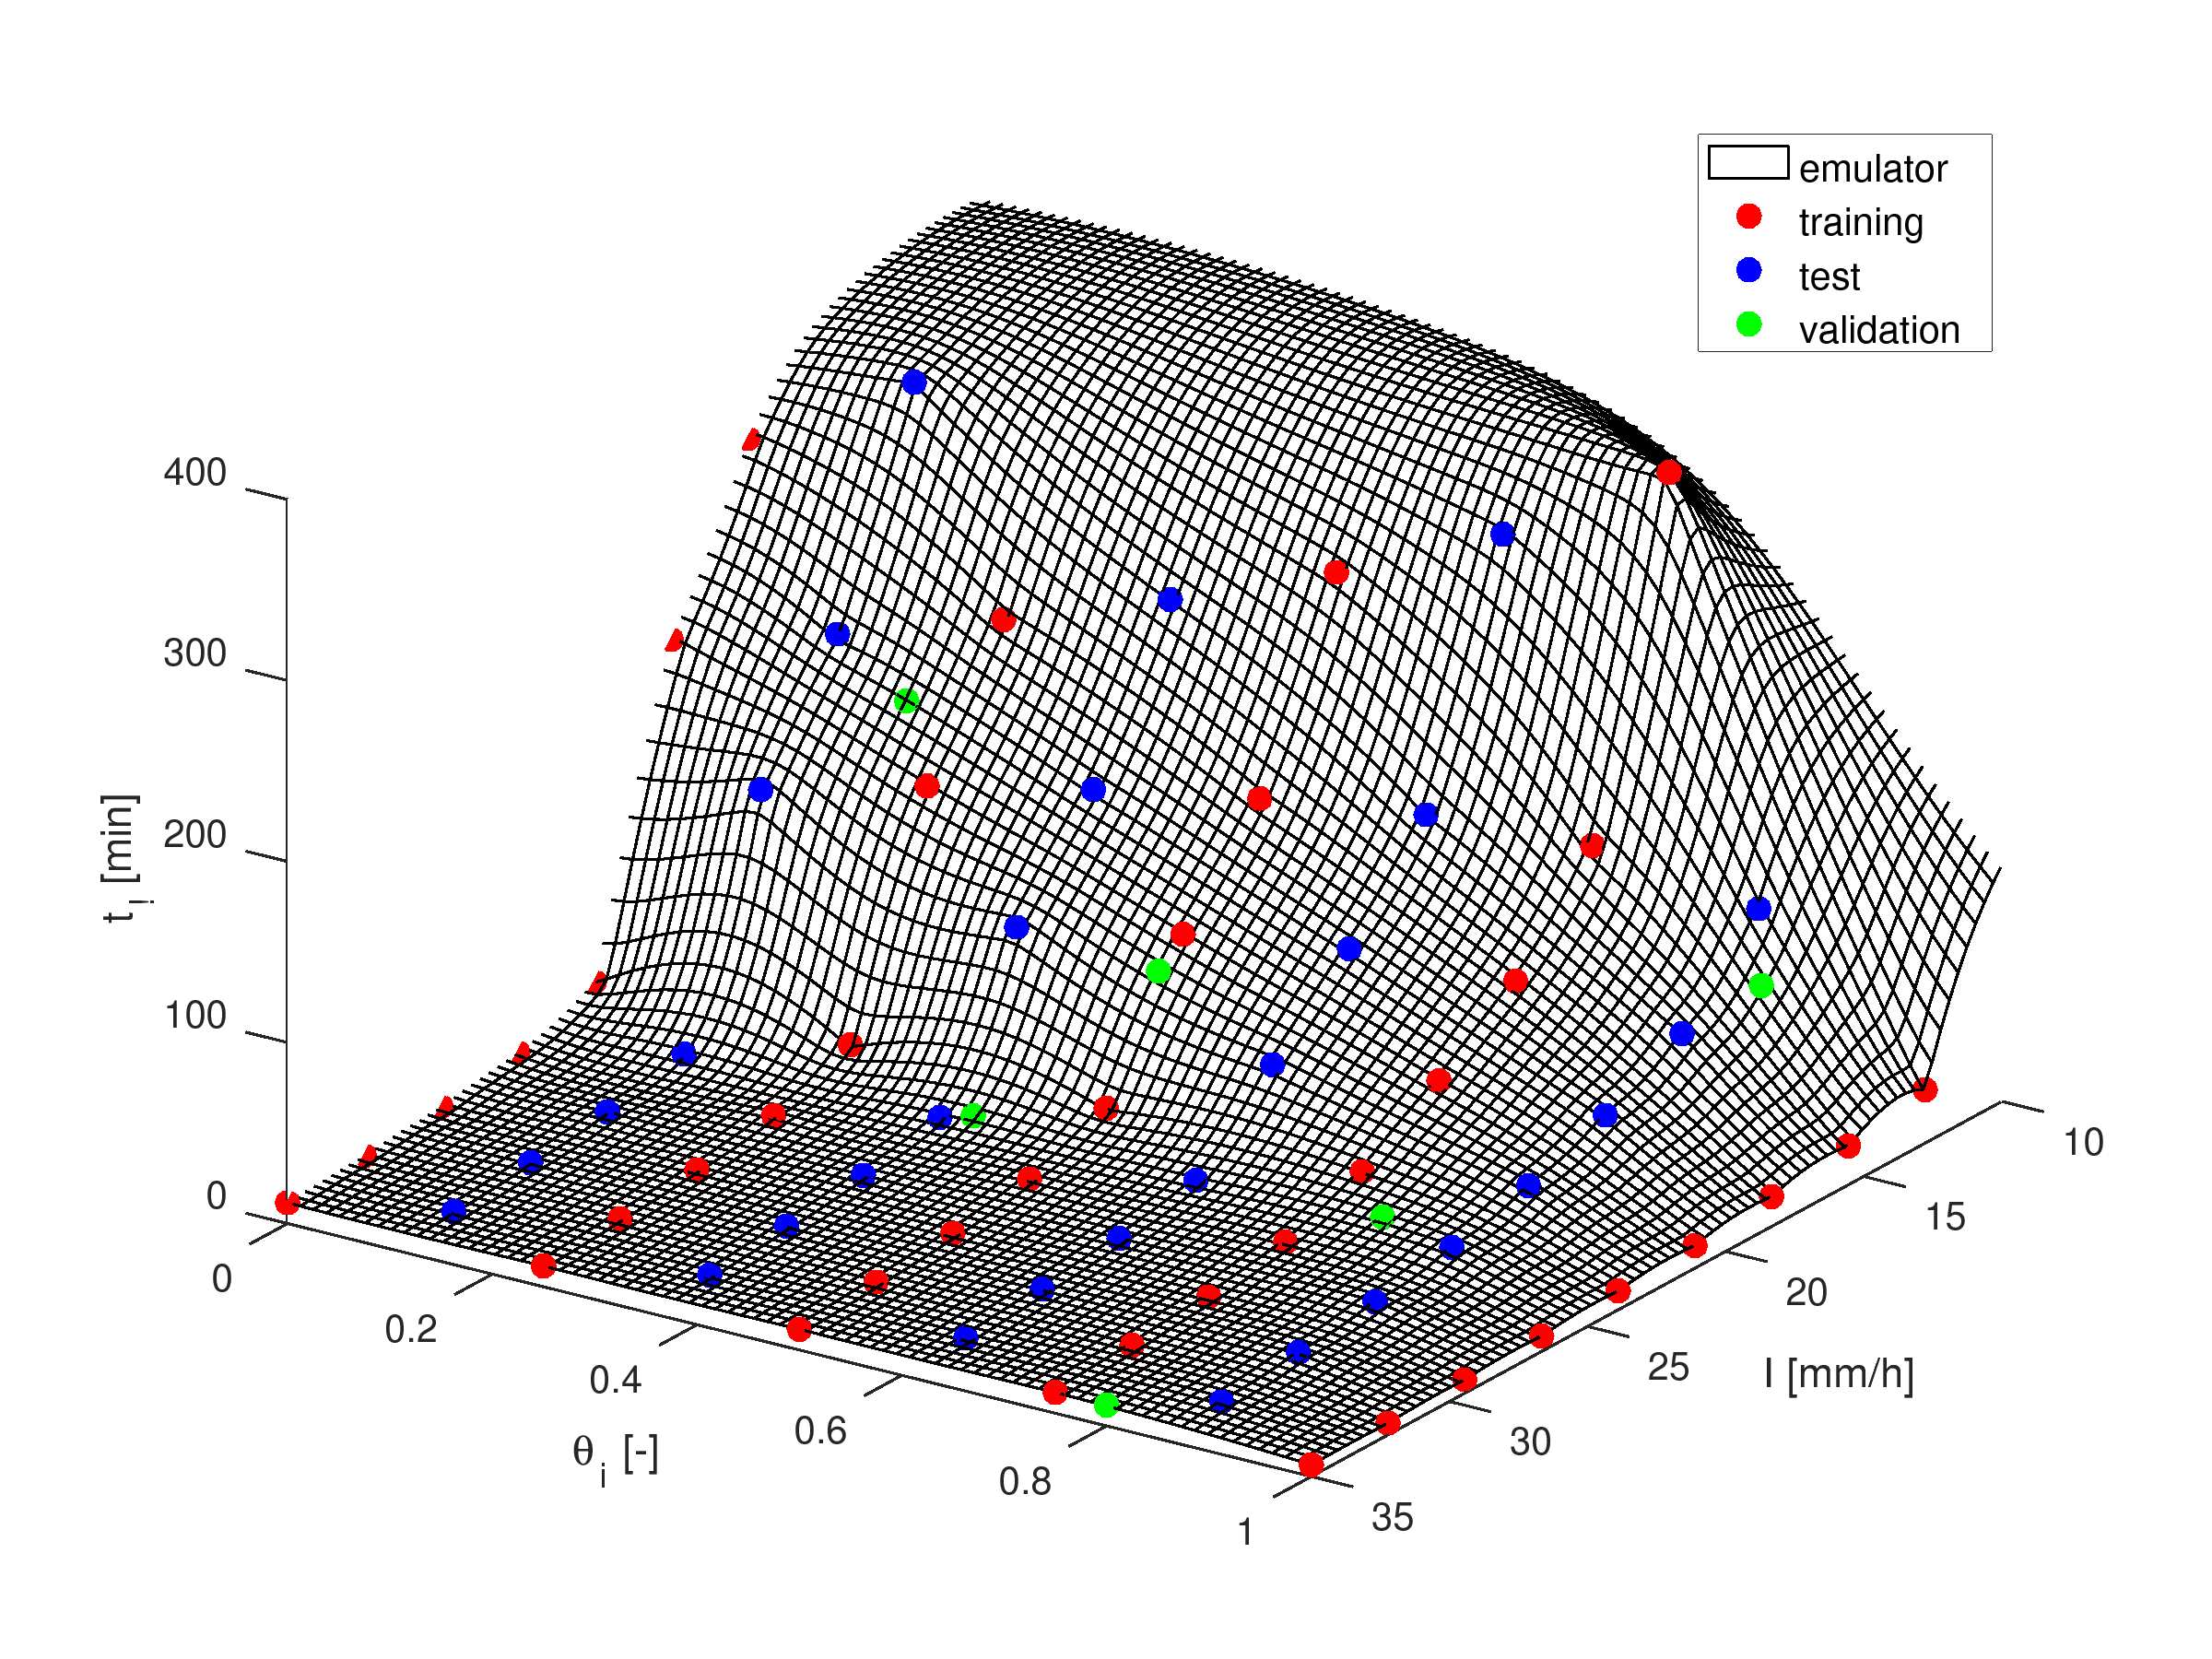
\includegraphics[width=0.7\textwidth]{Figures/emulator.png}
  \caption{Time-to-threshold emulator: training (red), test (blue) and validation (green) datasets and the emulator producing the intrapolation response.}
  \label{fig:regression_emulator}
\end{figure}


\begin{table}[htpb]
  \centering
  \caption{Emulator performance on \emph{test} and \emph{validation} data}
  \label{table label}
  \begin{tabular}{lcc}
    \toprule
     & \textbf{MAE [\si{\minute}, \si{\percent}]} & \textbf{RMSE [\si{\minute}, \si{\percent}]} \\
    \midrule
    \textbf{test} & val & val \\
    \textbf{validation} & val & val \\
    \bottomrule
  \end{tabular}
\end{table}

